\documentclass[12pt,oneside,a4paper]{report} 
\usepackage[utf8]{inputenc}
\usepackage[english]{babel}
\usepackage{graphicx}
\usepackage{fancyhdr}
\usepackage{tabularx}
\usepackage{supertabular}
\usepackage{comment}
\usepackage{hyperref}

% right header      
\rhead{Moon Games}
% left header
\lhead{Collab network protocol}
% centered footer
\cfoot{\thepage}
% use this style
\pagestyle{fancy}

% capter style
\makeatletter
\def\@makechapterhead#1{
{\parindent \z@ \raggedright \normalfont
\interlinepenalty\@M
\LARGE \bfseries \thechapter\ #1\par\nobreak
\vskip 30\p@
}}
\makeatother

%commands
\newcommand{\webURL}{\url{http://crpp.mgn.cz/}}


\begin{document}

% title page
\thispagestyle{empty}
\begin{center}

{\Huge Collaborative raster painting protocol}\\[50pt]

{\Huge CRPP}\\[100pt]

{\Large version 1.0}

\end{center}
\newpage

% content
\tableofcontents
\newpage

\part{Introduction}

\section{Licence}

All text of this document is licenced by GNU FDL version 1.3 or greater. Current version of licence text you can find on web address \url{http://www.gnu.org/copyleft/fdl.html}.

\section{Contact}

Author of this text is Moon Games group. Write us on mg@mgn.cz. Project web page \webURL{}.

\section{Document isn't final}

This document in development. It can containts mistakes, antagonism or incomplete informations. Take into account document development and call attention to authors for mistakes.

Text or his parts can be now in czech language. Please be patient and wait to translation. We are sorry. If you can help us with translation we will be pleasure with us cooperation. Please call attention to language mistakes.

\section{About document}

This document is part of \emph{CRPP} project, see \webURL for more informations.

\section{Introduction}

Document describes network protocol for collaborative painting (CRPP - Collaborative Raster Painting Protocol). We describing what we mean by ``collaborative painting" in first part of docuemnt (see \ref{part.colaborative-painting}). What its include and what not. Next part is about owns protocol (see \ref{part.protocol}).

\part{Collaborative painting}
\label{part.colaborative-painting}

Kolaborativním kreslením míníme sdílené kreslení mezi mnoha uživately v reálném čase. Sdílení by mělo probíhat v počítačové síťi.

\section{Stručný popis požadavků}

\begin{itemize}
	\item Je možné zakládat otevřené i zamčené místnosti.
	\item V každé místnosti je možné dynamicky přidávat a/i odebírat plátna. Plátna mají své jméno.
	\item U každého plátna lze dynamicky přidávat a/i odebírat vrstvy. Vrstvy lze pojmenovávat a měnit jejich pořadí.
	\item Do vrstev lze zakreslovat libovolný bitmapový obsah.
	\item Z vrstev je možné zcela, nebo částečně odmazávat (například pomocí gumy libovolného tvaru a krytí).
\end{itemize}


\part{Protokol}
\label{part.protocol}


\chapter{Obecný popis}

Protokol je rozdělen do dvou vzájemně nezávislých vrstev. To umožňuje oddělení funkcionality aplikačního síťového protokolu, přes který se posílají data, a vlastní datové struktury. Na obrázku \ref{picture.protocol_layers} jsou ilustrovány vrstvy protokolu.

\begin{figure}[h]
  \centering
  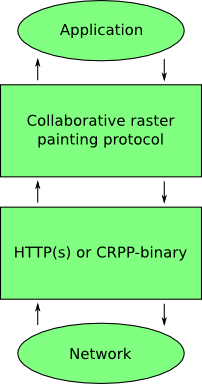
\includegraphics[width=0.30\textwidth]{diagrams/protocol_layers.png}
  \caption{Protocol layers diagram}
  \label{picture.protocol_layers}
\end{figure}

\subsection{Spodní vrstva}

Spodní vrstva se stará o spojení, jeho udržování, obnovování a fyzickou podobu přenášní dat. Je možné použít jeden ze dvou aplikačních protokolů (ve spodní vrstvě), a to HTTP(s) (viz \ref{chapter.http}), nebo CRPP-binary (viz \ref{chapter.crpp-binary}). Spodní vrstva komunikuje s vrchní tím, že jí předává respektive dostává monolitické bloky dat. Tyto bloky jsou stejné na obou stranách spojení. Viz diagram \ref{picture.monolithic_data_blocks}. Od okamžiku kdy bloky dat opustí vrstvu CRPP do jejich předání do této vrstvy na druhé straně spojení nesmí být změněno jejich pořadí (blok, který byl odeslán první, musí být jako první doručen).

\begin{figure}[h]
  \centering
  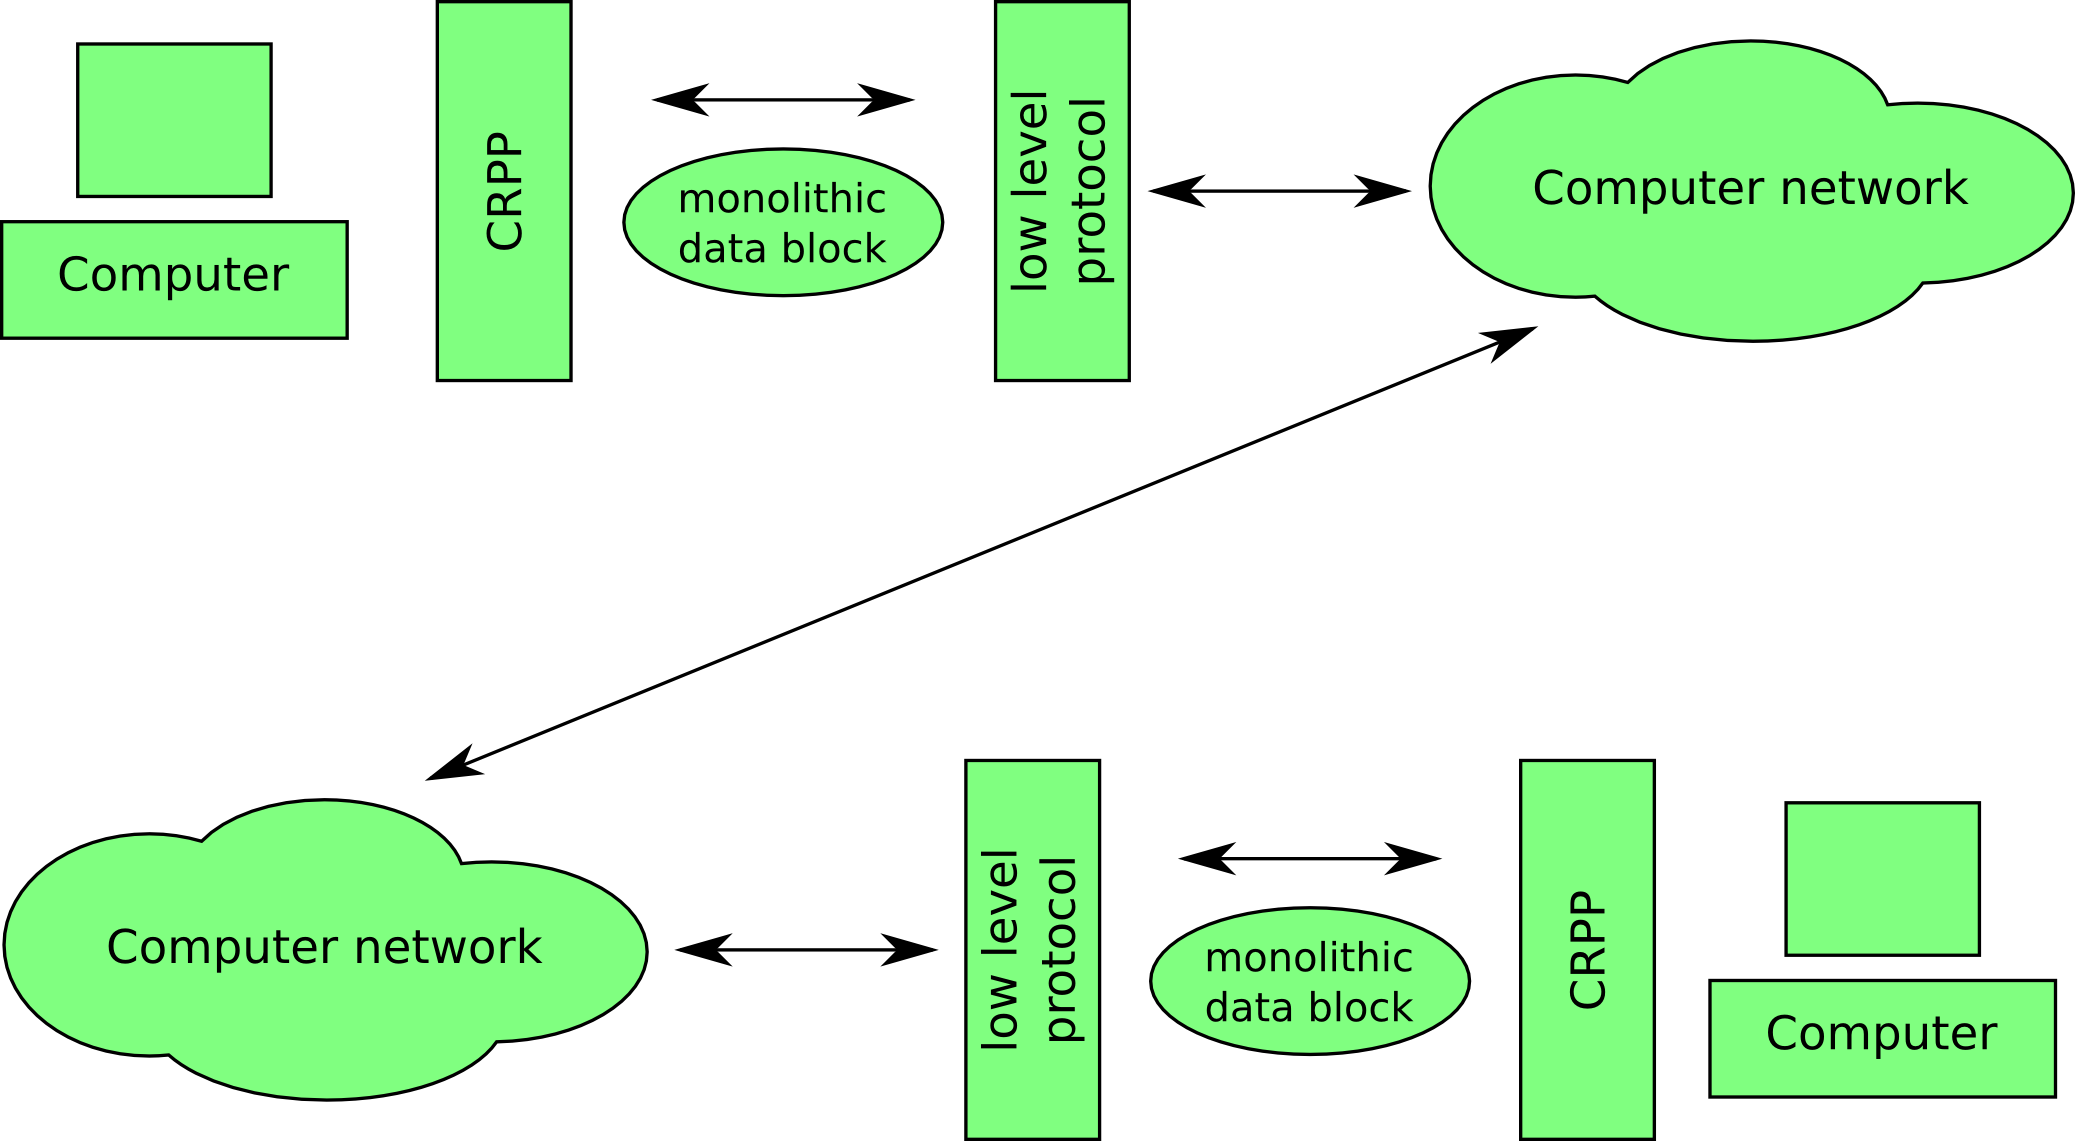
\includegraphics[width=0.80\textwidth]{diagrams/monolithic_data_blocks.png}
  \caption{Monolithic data blocks}
  \label{picture.monolithic_data_blocks}
\end{figure}

\subsection{Vrchní vrstva}

Vrchní vrstva monolitické bloky dat zpracovává. V kontextu vrchní vrstvy (vrstvy CRPP) se monolitické bloky dat označují jako ``message". Každá message je ucelený soubor dat (posloupnost bytů), který je možné jednotlivě zpracovat. Datová struktura a způsob zpracování message je popsáno v části \ref{text.collab_message}.

\chapter{CRPP-binary}
\label{chapter.crpp-binary}

% TODO: describe

\chapter{HTTP(s)}
\label{chapter.http}

% TODO: describe

\chapter{Collab message}
\label{text.collab_message}

CRPP message je posloupnost bytů. Každá message má význam příkazu (požadavku na vykonání nějaké funkce) a může obsahovat parametry.

\section{Data types}

Pokud není uvedeno jinak, tak všechny celočíselné hodnoty jsou bezeznaménkové.

\subsection{Unsigned integers}
\label{subsection.unsigned-integers}

Každý bit s hodnotou $1$ reprezentuje číslo $2^{p}$. Kde $p$ je pozice bitu (poslední bit -- v textu nejpravější -- posloupnosti má pozici $0$). Bity s hodnotou $0$ jsou rovny $0$.

\begin{equation}
\label{equation.unsigned-integers-sum}
\sum_{p = 0}^{n - 1} b_p 2^p
\end{equation}

$p$ je pozice bitu (poslední ma hodnotu 0, pak roste směrem k předcházejícím), $n$ je celkový počet bitů reprezentujících číslo, $b$ je hodnota bitu ($0$ nebo $1$).

Například posloupnost $00001010$ má hodnotu $10$ ($2^1 + 2^3$).

\subsection{Signed integers}

Hodnota znaménkového celého čísla je součet čísel $a$ a $b$ (tedy ${value} = a + b$). 

Hodnotu proměnné $a$ uručje vzorec $a = -2^{n - 1}$, kde $n$ je počet bitů reprezentujících číslo.

Hodnotu promměné $b$ určuje vzorec \ref{equation.unsigned-integers-sum} přičemž první bit není do vzorce vložen. Například posloupnost $10011$ by měla hodnotu $b = 2^0 + 2^1$ (není zahrnut první bit $1$). 

\subsection{Reálná čísla}

Reálná čísla jsou reprezentována podle standardu IEEE 754 ve 32 bitech.

\subsection{Logická hodnota} 

Logické hodnoty (boolean) jsou reprezentovány jedním bytem, kde samé nuly ($00000000$) reprezentují hodnotu \emph{false} a hodnota jedna ($00000001$) reprezentuje hodnotu \emph{true}. Ostatní hodnoty jsou považovány za nevalidní.

\subsection{Řetězce}

Veškerý text (řetězce zanků) je kódován jako UTF-8. V některých případech jako posloupnost ASCII znaků, to je ovšem vždy uvedeno. Všude je rozlišováno mezi malými a velkými písmeny (case sensitive).

\section{Message}

Message se skládá ze dvou částí: jejím příkazem a přídavnými daty (blocks). Příkaz reprezentují 4 ASCII znaky (4 byty). Bloky nemusí message obsahovat vůbec a může jich být neomezené množství. Jejich struktura je popsána v části \ref{text.collab_message.block}.

Obsah message je také ilustrován diagramem \ref{picture.message_structure}.

\begin{figure}[h]
  \centering
  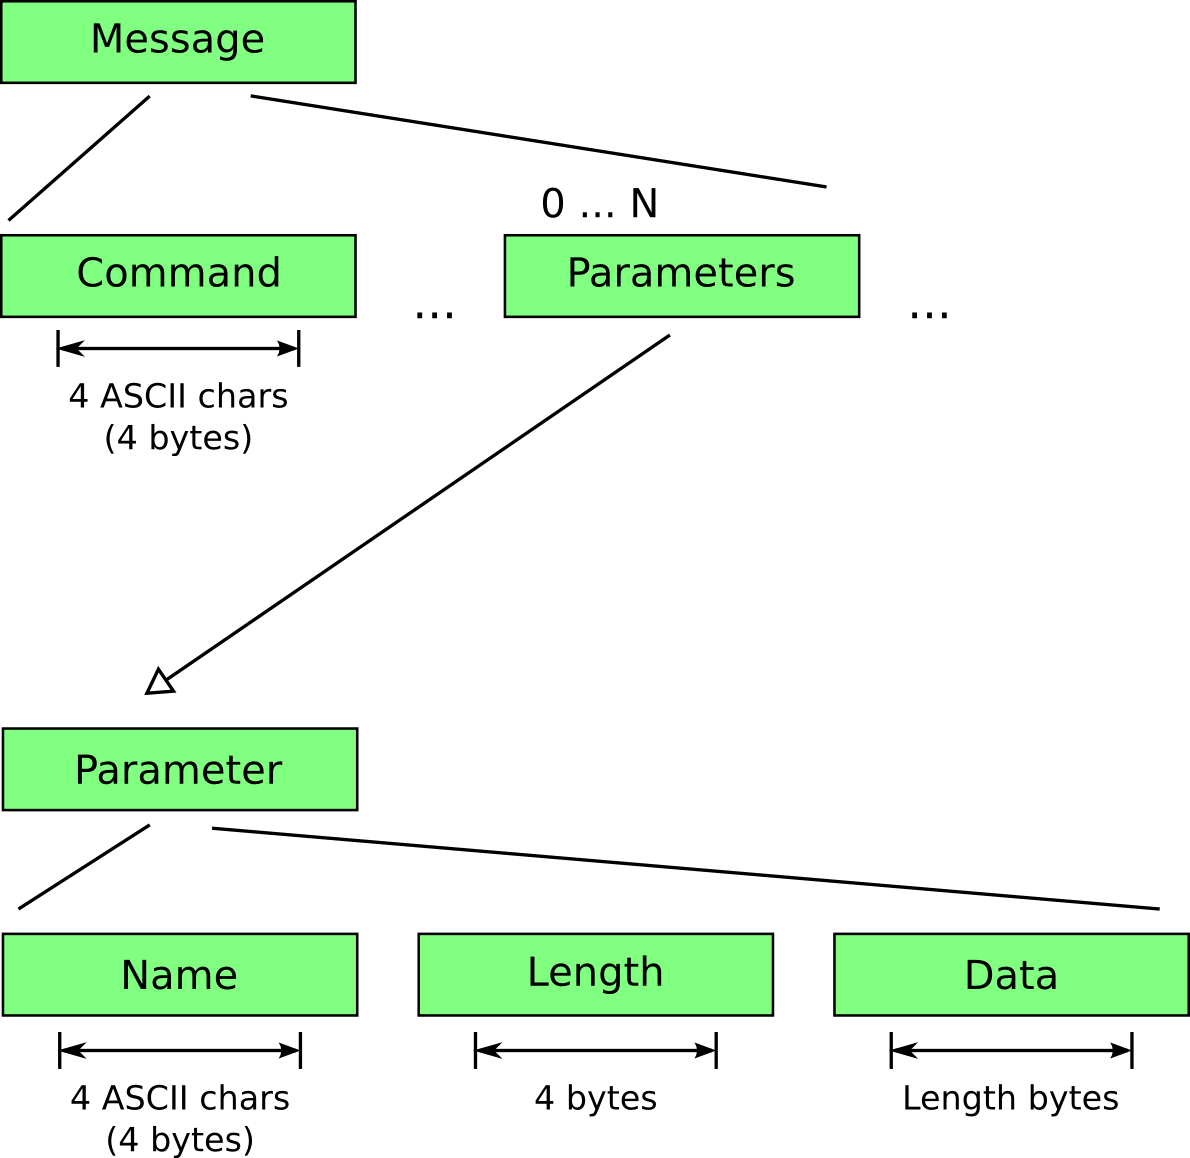
\includegraphics[width=0.80\textwidth]{diagrams/message_structure_diagram.png}
  \caption{Message structure diagram}
  \label{picture.message_structure}
\end{figure}

\section{Block}
\label{text.collab_message.block}

Block se dělí na tři části:

\begin{enumerate}
	\item block name (4\,{}B)
	\item block length (4\,{}B)
	\item block data (block length\,{}B)
\end{enumerate}

První část jsou 4 ASCII znaky (4 byty), které jednoznačně identifikují block. Následující 4 byty udávají jako neznaménkové celé číslo délku dat ($n$). Dalších $n$ bytů jsou data bloku. Data jsou interpretování různě podle toho v jakém příkazu je block obsažen a v jakém blocku jsou obsaženy data.

V části \ref{text.commands} jsou popsány jednotlivé commands, jejich blocks (parametry), význam a způsob zpracování.

\chapter{Commands}
\label{text.commands}

Příkazy se dělí na příchozí (posílá je server na klienty), odchozí (klienti je posílají na server) a obousměrné (posílají se na server i na klienta).

Seznam příkazů:

\begin{itemize}
	\item PANT -- paint
	\item LORD -- layers order
	\item ADDL -- add layer
	\item LNAM -- set layer name
\end{itemize}

\section{Příchozí}

\section{Odchozí}

\subsection{Add layer}

Přidá vrstvu do plátna. Obsahuje tyto bloky:

\begin{itemize}
	\item LPOS -- layer position
	\item LNAM -- layer name
	\item CNID -- canvas ID
\end{itemize}

\subsubsection{Server action}

Server vytvoří novou prázdnou vrstvu a zařadí jí do správné pozice. Poté odešle všem připojeným klientům nové layers order a pak name of this layer (set layer name).

\subsubsection{Blocks}

\paragraph{Layer position}

Obsahuje celočíselné čtyřbytové bezznaménkové číslo, které udává kolikátá v pořadí bude vrstva od spoda po přidání. Vrstva na pozici $0$ bude pod všemi ostatními. V případě, že je číslo větší než počet všech vrstev, bude vrstva přidána na vrch.

\paragraph{Layer name}

Obsahuje text s názvem vrstvy.

\paragraph{Canvas ID}

Obsahuje celočíslené bezznaménkové čtyřbytové číslo s ID plátna, do kterého má být vrstva přidána.

\section{Obousměrné}

\subsection{Paint}

Tento příkaz informuje o aktualizaci kreslícího plátna. Obsahuje tyto bloky:

\begin{itemize}
	\item UDTY -- update type
	\item UDID -- update ID
	\item LYID -- layer ID
	\item CNID -- canvas ID
	\item XCOR -- X coordinate
	\item YCOR -- Y coordinate
	\item UIMG -- update image data				
\end{itemize}

\subsubsection{Server action}

Server zakreslí update na příslušné místo a podé rozešle the same update (paint) to all connected users.

\subsubsection{Blocks}

\paragraph{Update type}
Update type je typ updatu a obsahuje čtyřbytové neznaménkové celočíselné číslo udávající typ updatu. Může nabívat hodnot $0$ a $1$, kde $0$ reprezentuje přidávácí update a $1$ mazací.

V případě přidávacího updatu se standartním (source over) algoritmem update nakreslí přes obrázek vrstvy. 

V případě odebíracího updatu se jen mění velikost alpha kanálu jednotlivých pixelů updatované vrstvy. Výsledná alpha každého pixelu $D_{a}$ se spočítá jako $D_{a} = S_{a} \cdot P_{a}$ kde $S_{a}$ značí alphu pixelu v updatovacím obrázku a $P_{a}$ značí alphu v v obrázku vrstvy před updatem. Všechny alphy ve výpočtu nabívají hodnot $0$ až $1$, takže je před výpočtem potřeba je převést ze standartní podoby $0$ až $255$ na tyto dělením číslem $255$ a po výpočtu převést zpátky násobením.

\paragraph{Update ID}
Obsahuje čtyřbytové neznaménkové celé číslo, které identifikuje tento update.

\paragraph{Layer ID}
Obsahuje čtyřbytové neznaménkové celé číslo, které identifikuje updatovanou vrstvu.

\paragraph{Canvas ID}
Obsahuje čtyřbytové neznaménkové celé číslo, které identifikuje updatované kreslící plátno (je tak možné kreslit na několik pláten).

\paragraph{X coordinate}
Obsahuje čtyřbytové neznaménkové celé číslo, které udává X souřadnici levého horního rohu updatu (kam se aplikuje updatovací obrázek).

\paragraph{Y coordinate}
Obsahuje čtyřbytové neznaménkové celé číslo, které udává Y souřadnici levého horního rohu updatu (kam se aplikuje updatovací obrázek).

\paragraph{Update image data}
Obsahuje binární data PNG obrázku typu ABGR. Viz http://www.w3.org/Graphics/PNG/. 

\end{document}